\chapter{Types}
\label{ch:types}
This Section defines Type Literals using EBNF and RegEx.
\section{Generic Types}
\label{sec:generic-types}
\subsection{Boolean}
\subsubsection{Boolean Data Type Definition}
The Boolean data type represents logical truth values. It has exactly two possible values: \texttt{True} and \texttt{False}. Booleans are used in conditional expressions, logical operations, and control flow decisions.

\subsubsection{Boolean Data Type Literals}
\begin{verbatim}
boolean_literal = "True" | "False"
\end{verbatim}
Boolean literals are case-sensitive: only \texttt{True} and \texttt{False} (capitalized) are valid. Lowercase \texttt{true}/\texttt{false} are not recognized as boolean literals.
\subsubsection{Boolean Data Type Casting and Coercion}
Boolean values can be coerced from other types:
\begin{itemize}
\item Int and real values coerce to \texttt{False} if zero, \texttt{True} otherwise
\item Strings coerce to \texttt{False} if empty, \texttt{True} otherwise
\item Lists and Sets coerce to \texttt{False} if empty, \texttt{True} otherwise
\item \texttt{None} coerces to \texttt{False}
\end{itemize}
Explicit conversion is not supported; boolean evaluation is implicit in conditional contexts.
\subsection{Null}
\subsubsection{Null Data Type Definition}
The Null data type represents the absence of a value. Null is a special singleton value that indicates ``no value''. Variables can be explicitly assigned null. Functions may return null to indicate failure or missing data.

\subsubsection{Null Data Type Literals}
\begin{verbatim}
null_literal = "null"
\end{verbatim}

\begin{itemize}
\item \texttt{null} is case-sensitive: only lowercase \texttt{null} is valid.
\item \texttt{null} is distinct from \texttt{None}. \texttt{None} is the implicit return value of functions that do not explicitly return; \texttt{null} explicitly represents the absence of a value.
\item Accessing a member or index of \texttt{null} raises a \texttt{Runtime Error} unless the safe access operator (\texttt{?.}) or safe indexing operator (\texttt{?[]}) is used.
\end{itemize}

\subsubsection{Null Coercion}
\begin{itemize}
\item \texttt{null} coerces to \texttt{False} in boolean contexts.
\item \texttt{null} coerces to \texttt{0} in numeric contexts (raises \texttt{Type Error} for explicit casting).
\end{itemize}

\subsubsection{Null Coalescing}
The null coalescing operator \texttt{??} returns the left operand if it is not \texttt{null}, otherwise the right operand:
\begin{verbatim}
a ?? b   Returns a if a is not null, else b
\end{verbatim}

\subsubsection{Safe Access}
The safe member access operator \texttt{?.} returns \texttt{null} if the left operand is \texttt{null}, instead of raising a \texttt{Runtime Error}:
\begin{verbatim}
obj?.member   Returns obj.member if obj is not null, else null
\end{verbatim}

The safe indexing operator \texttt{?[]} returns \texttt{null} if the left operand is \texttt{null}:
\begin{verbatim}
array?[index]   Returns array[index] if array is not null, else null
\end{verbatim}

\subsubsection{Null Examples}
\begin{verbatim}
$x [int]= null         #c# $x is null
$y = $x ?? 5           #c# $y = 5 (null coalescing)
$obj?.property         #c# returns null if $obj is null
$arr?[0]               #c# returns null if $arr is null
\end{verbatim}

\subsection{Integer}
\subsubsection{Integer Data Type Definition}
The Integer data type represents whole numbers (elements of $\mathbb{Z}$). Integers support standard arithmetic operations and can express values from very large negative to very large positive using SI decimal prefixes (kilo and above).
\subsubsection{Integer Data Type Literals}
Integer literals can be expressed in multiple formats:
\begin{verbatim}
EBNF:
int_literal = decimal_int | binary_literal 
            | octal_literal | hex_literal | bin_exp_int

decimal_int = ["+" | "-"], digit, {digit}, [si_prefix | bin_prefix]

binary_literal   = "0b", bindigit, {bindigit}, [si_prefix | bin_prefix]
octal_literal    = "0o", octdigit, {octdigit}, [si_prefix | bin_prefix]
hex_literal      = "0x", hexdigit, {hexdigit}, [si_prefix | bin_prefix]

bin_exp_int = ["+" | "-"], digit, {digit}, ("w" | "W"), "+", digit, {digit}

si_prefix = "q" | "r" | "y" | "z" | "a" | "f" | "p" | "n" | "u" | "m"
          | "c" | "d" | "h" | "da"
          | "k" | "M" | "G" | "T" | "P" | "E" | "Z" | "Y" | "R" | "Q"

bin_prefix = "ki" | "Mi" | "Gi" | "Ti" | "Pi" | "Ei" | "Zi" | "Yi" | "Ri" | "Qi"

RegEx:
digit     = [0-9]
bindigit  = [01]
octdigit  = [0-7]
hexdigit  = [0-9a-fA-F]
\end{verbatim}

SI prefixes $\geq$ k and scientific notation produce integers when the result is numerically equal to an integer:
\begin{verbatim}
6.2k    #c# = 6200 (int)
1M      #c# = 1000000 (int)
-5e9    #c# = -5000000000 (int, exact)
5e-1    #c# = 0.5 (real, not exact)
4Q      #c# = 4e30 (int)
\end{verbatim}

Binary (IEC 60027-2) prefixes produce integers by multiplying with powers of 2:
\begin{verbatim}
1ki     #c# = 1024 (2^10)
4Mi     #c# = 4194304 (2^20)
2Gi     #c# = 2147483648 (2^30)
1Ti     #c# = 1099511627776 (2^40)
0x10ki  #c# = 16384 (0x10 * 1024)
\end{verbatim}

Binary, octal, and hex literals always produce integers:
\begin{verbatim}
0x10    #c# = 16
0b1010  #c# = 10
0o17    #c# = 15
\end{verbatim}

Binary exponent notation uses \texttt{w}/\texttt{W} (mnemonic: \textbf{w}ide) to multiply a mantissa by $2^{\text{exponent}}$. When the mantissa has no decimal point and the exponent is $\geq$ 0, the result is an integer:
\begin{verbatim}
4w10    #c# = 4096 (4 * 2^10)
5W1     #c# = 10 (5 * 2^1)
1w0     #c# = 1 (1 * 2^0)
\end{verbatim}

\subsubsection{Integer Data Type Casting and Coercion}
Integers can be coerced from other types:
\begin{itemize}
\item Booleans coerce to \texttt{0} (False) or \texttt{1} (True)
\item Numeric strings with no decimal point are parsed as integers (e.g., \texttt{"42"} becomes \texttt{42})
\item \texttt{real} values are truncated (e.g., \texttt{3.7} cast to \texttt{int} becomes \texttt{3})
\end{itemize}

\subsection{Real}
\subsubsection{Real Data Type Definition}
The Real data type represents floating-point numbers (elements of $\mathbb{R}$). Reals support standard arithmetic operations and can express values from very small (quecto-scale, $10^{-30}$) to very large (quetta-scale, $10^{30}$) using SI decimal prefixes.
\subsubsection{Real Data Type Literals}
Real literals can be expressed in multiple formats:
\begin{verbatim}
EBNF:
real_literal = decimal_real | scientific_real | bin_exp_literal

decimal_real   = ["+" | "-"], digit, {digit}, ".", {digit}, [si_prefix]
               | ["+" | "-"], ".", digit, {digit}, [si_prefix]

scientific_real = ["+" | "-"], digit, {digit}, 
                  ["." , {digit}], ("e" | "E"), 
                  ["+" | "-"], digit, {digit}
               | ["+" | "-"], ".", digit, {digit}, 
                  ("e" | "E"), 
                  ["+" | "-"], digit, {digit}

bin_exp_literal = ["+" | "-"], digit, {digit}, ["." , {digit}],
                  ("w" | "W"), ["+" | "-"], digit, {digit}
               | ["+" | "-"], ".", digit, {digit},
                  ("w" | "W"), ["+" | "-"], digit, {digit}
\end{verbatim}

A literal with a decimal point or scientific notation produces a real, even if the fractional part is zero:
\begin{verbatim}
3.14    #c# = 3.14 (real)
42.0    #c# = 42.0 (real)
42e0    #c# = 42.0 (real)
.4      #c# = 0.4 (real)
.5e2    #c# = 50.0 (real, leading-dot scientific)
2e-6    #c# = 0.000002 (real)
\end{verbatim}

Binary exponent notation produces a real when the mantissa has a decimal point or the exponent is negative:
\begin{verbatim}
1w-3    #c# = 0.125 (1 * 2^-3)
3.5w2   #c# = 14.0 (3.5 * 2^2, real because decimal mantissa)
.5w-1   #c# = 0.25 (0.5 * 2^-1)
\end{verbatim}

SI prefixes below k produce reals:
\begin{verbatim}
100n    #c# = 0.0000001 (real)
1m      #c# = 0.001 (real)
5c      #c# = 0.05 (real)
\end{verbatim}

The full SI prefix table:
\begin{center}
\begin{tabular}{lll@{\hspace{3em}}lll}
\hline
Prefix & Value & Name & Prefix & Value & Name \\
\hline
\multicolumn{3}{l}{\textit{Sub-unit ($< 1$)}} & \multicolumn{3}{l}{\textit{Multiple ($\geq 1$)}} \\
q  & $10^{-30}$ & quecto  & k  & $10^{3}$  & kilo  \\
r  & $10^{-27}$ & ronto   & M  & $10^{6}$  & mega  \\
y  & $10^{-24}$ & yocto   & G  & $10^{9}$  & giga  \\
z  & $10^{-21}$ & zepto   & T  & $10^{12}$ & tera  \\
a  & $10^{-18}$ & atto    & P  & $10^{15}$ & peta  \\
f  & $10^{-15}$ & femto   & E  & $10^{18}$ & exa   \\
p  & $10^{-12}$ & pico    & Z  & $10^{21}$ & zetta \\
n  & $10^{-9}$  & nano    & Y  & $10^{24}$ & yotta \\
u  & $10^{-6}$  & micro   & R  & $10^{27}$ & ronna \\
m  & $10^{-3}$  & milli   & Q  & $10^{30}$ & quetta \\
c  & $10^{-2}$  & centi   & h  & $10^{2}$  & hecto  \\
d  & $10^{-1}$  & deci    & da & $10^{1}$  & deca   \\
\hline
\end{tabular}
\end{center}

Prefixes $\geq$ k produce integers. Prefixes $<$ k produce reals.

The full binary (IEC 60027-2) prefix table:
\begin{center}
\begin{tabular}{llll}
\hline
Prefix & Value & Decimal & Name \\
\hline
ki & $2^{10}$  & $1\,024$                    & kibi  \\
Mi & $2^{20}$  & $1\,048\,576$               & mebi  \\
Gi & $2^{30}$  & $1\,073\,741\,824$          & gibi  \\
Ti & $2^{40}$  & $1\,099\,511\,627\,776$     & tebi  \\
Pi & $2^{50}$  & $1.1259 \times 10^{15}$     & pebi  \\
Ei & $2^{60}$  & $1.1529 \times 10^{18}$     & exbi  \\
Zi & $2^{70}$  & $1.1806 \times 10^{21}$     & zebi  \\
Yi & $2^{80}$  & $1.2089 \times 10^{24}$     & yobi  \\
Ri & $2^{90}$  & $1.2379 \times 10^{27}$     & robi  \\
Qi & $2^{100}$ & $1.2677 \times 10^{30}$     & quebi \\
\hline
\end{tabular}
\end{center}

Binary prefixes always produce integers.

\subsubsection{Real Data Type Casting and Coercion}
Reals can be coerced from other types:
\begin{itemize}
\item Integers coerce to real (e.g., \texttt{real(5)} becomes \texttt{5.0})
\item Booleans coerce to \texttt{0.0} (False) or \texttt{1.0} (True)
\item Numeric strings with a decimal point are parsed as reals (e.g., \texttt{"3.14"} becomes \texttt{3.14})
\item Non-numeric strings raise a type error
\end{itemize}
Lists of ints or reals can be passed to mathematical functions, which operate element-wise.
\subsection{Complex}
\subsubsection{Complex Data Type Definition}
The Complex data type represents complex numbers (elements of $\mathbb{C}$). A complex number has a real part and an imaginary part, and can be expressed in rectangular or polar form.

\paragraph{Type Hierarchy}
\begin{center}
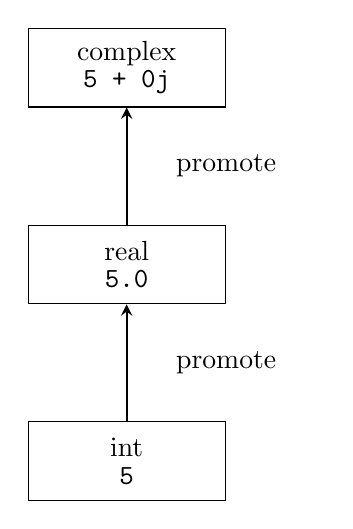
\begin{tikzpicture}[>=stealth, node distance=2.5cm, every node/.style={draw, rectangle, minimum width=2.5cm, minimum height=1cm, align=center}]
  \node (complex) {complex\\[-2pt]\texttt{5 + 0j}};
  \node (real) [below of=complex] {real\\[-2pt]\texttt{5.0}};
  \node (int) [below of=real] {int\\[-2pt]\texttt{5}};
  \draw[->, thick] (int) -- node[right, draw=none] {promote} (real);
  \draw[->, thick] (real) -- node[right, draw=none] {promote} (complex);
\end{tikzpicture}
\end{center}

Auto-promotion is implicit and lossless: an \texttt{int} can be used wherever a \texttt{real} is expected, and both can be used wherever a \texttt{complex} is expected.

\subsubsection{Complex Data Type Literals}
\begin{verbatim}
EBNF:
complex_literal = rectangular_literal | polar_literal

rectangular_literal = ["+" | "-"], number, ["+", number, "j"] 
                    | ["+" | "-"], number, "-", number, "j"
                    | ["+" | "-"], number, "j"

polar_literal = number, "<|", number
\end{verbatim}

The \texttt{j} suffix on a number creates a complex literal. The \texttt{<|} operator creates a polar literal (magnitude <| angle in radians).

\paragraph{Rectangular Form}
\begin{verbatim}
3 + 4j        #c# real=3, imag=4
-2 - 7j       #c# real=-2, imag=-7
5j            #c# real=0, imag=5
3             #c# real=3, imag=0 (int promoted to complex)
3.14 + 2.71j  #c# real=3.14, imag=2.71
\end{verbatim}

Note: \texttt{3 + 4j} is a single complex literal in rectangular form. The \texttt{+} is part of the literal, not the addition operator.

\paragraph{Polar Form}
\begin{verbatim}
2 <| 1.5708    #c# magnitude=2, angle=pi/2 (radians)
1 <| 0         #c# magnitude=1, angle=0 (real number 1)
1 <| 3.14159   #c# magnitude=1, angle=pi (real number -1)
\end{verbatim}

\subsubsection{Complex Data Type Casting and Coercion}
\begin{itemize}
\item \texttt{int} promotes to \texttt{complex}: \texttt{5} becomes \texttt{5 + 0j}
\item \texttt{real} promotes to \texttt{complex}: \texttt{3.14} becomes \texttt{3.14 + 0j}
\item Mixed operations (\texttt{int + complex}, \texttt{real + complex}) produce \texttt{complex}
\item \texttt{complex} cannot be coerced to \texttt{real} or \texttt{int} (use \texttt{real()} or \texttt{int()} to extract parts)
\item Booleans coerce to \texttt{complex}: \texttt{True} becomes \texttt{1 + 0j}
\item Lists of complex can be passed to mathematical functions, which operate element-wise
\end{itemize}

\subsubsection{Complex Components}
The real and imaginary parts of a complex number are accessed via functions:
\begin{verbatim}
real($z)   #c# Returns the real part (real)
imag($z)   #c# Returns the imaginary part (real)
\end{verbatim}
See Section~\ref{sec:complex_functions} for full documentation.
\subsection{Set}
\subsubsection{Set Data Type Definition}
A Set is an unordered collection of unique elements. Sets can contain any data type:
\begin{itemize}
\item Integers and reals (numbers)
\item Strings
\item Booleans
\item Lists
\item Parts
\item Connections
\item Pins
\item Nets
\end{itemize}

Sets containing mixed types are allowed. Duplicate elements are automatically removed. Sets support standard set algebra operations (union, intersection, difference, subset, element-of).

\subsubsection{Set Data Type Literals}
\begin{verbatim}
EBNF:
set_literal = "{", [ { data, ","}, data ], "}"
            | "{", range_spec, "}"
\end{verbatim}

Examples:
\begin{verbatim}
$numbers [set]= { 1, 2, 3, 4, 5 }
$mixed [set]= { 1, "hello", True, Q1 }
$parts [set]= { Q1, Q2, R3 }
\end{verbatim}

Sets also support range generation using the same syntax as lists:
\begin{verbatim}
{start:increment:end}       #c# explicit increment
{start:end}                 #c# increment defaults to 1
{start|end|count}           #c# evenly spaced, count elements
{start >: increment :< end} #c# exclusive start and end (colon)
{start >|< end | count}     #c# exclusive start and end (pipe)
\end{verbatim}
Examples:
\begin{verbatim}
$evens [set]= {0:2:10}         #c# {0, 2, 4, 6, 8, 10}
$range [set]= {0:5}            #c# {0, 1, 2, 3, 4, 5}
$lin   [set]= {0|1|5}          #c# {0, 0.25, 0.5, 0.75, 1}
$excl1 [set]= {0>:4}           #c# {1, 2, 3, 4}
$excl2 [set]= {0:<5}           #c# {0, 1, 2, 3, 4}
$excl3 [set]= {0>:<5}          #c# {1, 2, 3, 4}
$excl4 [set]= {0>:2:<10}       #c# {2, 4, 6, 8}
$excl5 [set]= {0>|<1|5}        #c# {0.1667, 0.3333, 0.5, 0.6667, 0.8333}
\end{verbatim}

Note: since sets are unordered and unique, duplicates within a range are silently ignored. For example, \texttt{\{0:0.3:1\}} produces \texttt{\{0, 0.3, 0.6, 0.9\}} with no duplicate \texttt{0} entries.

\subsubsection{Set Data Type Casting and Coercion}
Sets can be created from Lists using the \texttt{f.set()} function. When converting a List to a Set, duplicate elements are removed and order is lost.\\
Example:
\begin{verbatim}
$my_list [list]= [ 1, 2, 2, 3, 3, 3 ]
$my_set [set]= f.set( $my_list )  #c# { 1, 2, 3 }
\end{verbatim}
Sets can be converted to Lists using the \texttt{f.list()} function. The order of elements in the resulting List is determined by the order they appear in the global set \texttt{*e}.
\subsection{String}
\subsubsection{String Data Type Definition}
The String data type represents textual data. Strings can be delimited by single or double quotes, and support escape sequences. Long strings (multi-line) are delimited by triple quotes. Raw strings (suffix \texttt{R}) disable escape processing.
\subsubsection{String Data Type Literals}
\begin{verbatim}
EBNF:
string_literal = long_string | short_string
short_string   =   '"', {short_string_item_I},  '"', ["R"]   |
                   "'", {short_string_item_II}, "'", ["R"]
long_string    = '"""',  {long_string_item_I},  '"""' |
                 "'''",  {long_string_item_II}, "'''"

RegEx:
short_string_item_I  = [^"\\\n]|(\\.)
short_string_item_II = [^'\\\n]|(\\.)
 long_string_item_I  = [^"\\]|(\\.)
 long_string_item_II = [^'\\]|(\\.)
\end{verbatim}

\paragraph{Escape Sequences}
\begin{center}
\begin{tabular}{|l|l|l|}
\hline
\textbf{Sequence} & \textbf{Name} & \textbf{Description} \\
\hline
\texttt{\textbackslash n} & Newline & Line feed (U+000A) \\
\texttt{\textbackslash t} & Tab & Horizontal tab (U+0009) \\
\texttt{\textbackslash r} & Carriage Return & CR (U+000D) \\
\texttt{\textbackslash 0} & Null & Null character (U+0000) \\
\texttt{\textbackslash\textbackslash} & Backslash & Literal backslash \\
\texttt{\textbackslash"} & Double Quote & Literal double quote inside \texttt{"..."} \\
\texttt{\textbackslash'} & Single Quote & Literal single quote inside \texttt{'...'} \\
\texttt{\textbackslash r\textbackslash n} & CRLF & Windows line ending (CR+LF) \\
\texttt{\textbackslash xHH} & Hex Byte & Two-digit hex, e.g. \texttt{\textbackslash x41} = \texttt{A} \\
\texttt{\textbackslash uHHHH} & Unicode & 4-digit codepoint, e.g. \texttt{\textbackslash u0041} = \texttt{A} \\
\texttt{\textbackslash UHHHHHHHH} & Unicode & 8-digit codepoint for supplementary chars \\
\texttt{\textbackslash\textless{}other\textgreater{}} & Literal & Unknown sequences remain as-is (e.g. \texttt{\textbackslash q} $\rightarrow$ \texttt{\textbackslash q}) \\
\hline
\end{tabular}
\end{center}

\paragraph{Raw Strings}
Append \texttt{R} to the closing quote to disable escape processing. Content is literal. Useful for file paths, regex patterns, and any string where backslashes should not be interpreted.
\begin{verbatim}
$path [string]= "C:\Users\test\file.txt"R   #c# Literal: C:\Users\test\file.txt
$regex [string]= '\d+\.\d+'R              #c# Literal: \d+\.\d+
$normal [string]= "Line1\nLine2"           #c# Contains actual newline
$raw [string]= "Line1\nLine2"R            #c# Literal: Line1\nLine2
\end{verbatim}

\subsubsection{String Data Type Casting and Coercion}
Strings can be created from other types using the \texttt{f.str()} function, which concatenates all arguments into a single string.\\
Example:
\begin{verbatim}
$msg [string]= f.str( "The value is ", 42, 
    " and color is ", "red" )
#c# $msg = "The value is 42 and color is red"
\end{verbatim}
Additional string functions include \texttt{f.upperc()} (uppercase), \texttt{f.lowerc()} (lowercase), and \texttt{f.format()} (formatted output).
\subsection{List}
\subsubsection{List Data Type Definition}
The List data type represents an ordered, indexed collection of objects. Lists support 0-based indexing, slicing, and can contain elements of different types. Lists are mutable and can be dynamically resized. Assignment creates a copy (not a reference).
\subsubsection{List Data Type Literals}
\begin{verbatim}
EBNF:
list_literal = "[", [{ data, "," }, data], "]"
             | "[", range_spec, "]"

set_literal = "{", [ { data, ","}, data ], "}"
            | "{", range_spec, "}"

range_spec  = expression, [">"], ":", expression, [":", ["<"], expression]
            | expression, [">"], "|", ["<"], expression, "|", expression

slice       = [expression], ":", [expression], [":", expression]

boolean_indexing = expression, "[", boolean_expression, "]"

tensor_indexing  = expression, "[", indexing_expr, "]"

indexing_expr    = expression                        # single index or boolean
                 | expression, ",", expression       # multi-dimensional
                 | slice_spec                        # slice
                 | list_literal                      # index list
                 | "...", [",", indexing_expr]        # ellipsis

slice_spec       = [expression], ":", [expression], [":", ["-", ] expression]

safe_tensor_indexing = expression, "?[", indexing_expr, "]"

reshape     = ".", "reshape", "(", int, {",", int}, ")"

assignable  = variable
            | variable, "[", indexing_expr, "]"
            | variable, "?[", indexing_expr, "]"
\end{verbatim}

\paragraph{Exclusive Ranges}
The colon and pipe range syntax supports optional exclusive boundary modifiers. The \texttt{>} modifier (placed before \texttt{:} or \texttt{|}) excludes the start value. The \texttt{<} modifier (placed after \texttt{:} or \texttt{|}) excludes the end value. Both modifiers can be combined.

For colon ranges, exclusive boundaries shift the first or last element by one step:
\begin{itemize}
\item \texttt{[start >: end]} --- exclusive start: elements begin at \texttt{start + increment} (default increment is 1)
\item \texttt{[start :< end]} --- exclusive end: elements stop at \texttt{end - increment}
\item \texttt{[start >:< end]} --- exclusive both
\item \texttt{[start >: increment :< end]} --- exclusive both with explicit increment
\end{itemize}

For pipe ranges, exclusive boundaries change the step calculation:
\begin{itemize}
\item \texttt{[start | end | count]} --- inclusive: step $= \frac{\text{end} - \text{start}}{\text{count} - 1}$, requires \texttt{count} $\geq 2$
\item \texttt{[start >| end | count]} --- exclusive start: step $= \frac{\text{end} - \text{start}}{\text{count}}$, first element is \texttt{start + step}
\item \texttt{[start |< end | count]} --- exclusive end: step $= \frac{\text{end} - \text{start}}{\text{count}}$, last element is \texttt{end - step}
\item \texttt{[start >|< end | count]} --- exclusive both: step $= \frac{\text{end} - \text{start}}{\text{count} + 1}$, first element is \texttt{start + step}
\end{itemize}

\subsubsection{List Data Type Casting and Coercion}
Lists can be created from Sets using the \texttt{f.list()} function. The order is determined by the element order in \texttt{*e}.\\
Lists support range generation using the syntax:
\begin{verbatim}
[start:increment:end]       #c# explicit increment
[start:end]                 #c# increment defaults to 1
[start|end|count]           #c# evenly spaced, count elements
[start >: increment :< end] #c# exclusive start and end (colon)
[start >|< end | count]     #c# exclusive start and end (pipe)
\end{verbatim}
Examples:
\begin{verbatim}
$r1 [list]= [0:2:10]         #c# [0, 2, 4, 6, 8, 10]
$r2 [list]= [0:5]            #c# [0, 1, 2, 3, 4, 5]
$r3 [list]= [0|1|5]          #c# [0, 0.25, 0.5, 0.75, 1]
$r4 [list]= [0>:4]           #c# [1, 2, 3, 4]
$r5 [list]= [0:<5]           #c# [0, 1, 2, 3, 4]
$r6 [list]= [0>:<5]          #c# [1, 2, 3, 4]
$r7 [list]= [0>:2:<10]       #c# [2, 4, 6, 8]
$r8 [list]= [0>|<1|5]        #c# [0.1667, 0.3333, 0.5, 0.6667, 0.8333]
\end{verbatim}
\subsection{Tensor}
\paragraph{Definition}
A Tensor is a subtype of List that is \textbf{rectangular} (all sublists have the same length) and contains only \textbf{numeric} values (\texttt{bool}, \texttt{int}, \texttt{real}, or \texttt{complex}). Tensors are explicitly typed using the \texttt{[tensor]} annotation or the pipe-prefixed literal syntax.

\paragraph{Historical Note}
Tensors were previously called ``ndarrays'' (N-dimensional arrays) in earlier versions of this specification. The name has been changed to ``tensor'' to better reflect the mathematical concept and to distinguish the explicit type from the old auto-detected behavior.

\paragraph{Type Hierarchy}
Tensor is a subtype of List:
\begin{itemize}
\item A Tensor IS-A List: all list operations work on tensors
\item A List IS NOT necessarily a Tensor: lists may have mixed types or non-rectangular shapes
\item Tensor elements must be numeric (\texttt{bool}, \texttt{int}, \texttt{real}, or \texttt{complex})
\item Tensor shape is fixed at creation time
\end{itemize}

\subsubsection{Tensor Data Type Literals}
\begin{verbatim}
EBNF:
  tensor_literal = "|", "[", [{ data, "," }, data], "]"
  | "|", "[", range_spec, "]"
  \end{verbatim}
  The pipe prefix \texttt{|} distinguishes tensor literals from list literals. Tensors are explicitly typed and support the same range syntax as lists.

  \paragraph{Warning}
  \textbf{Incorrect syntax:} \texttt{|[]|} --- this will cause immediate program termination.
  \textbf{Correct syntax:} \texttt{|[]} --- the pipe prefix is only at the opening bracket.
  \begin{itemize}
  \item \texttt{|[]} --- valid empty tensor
  \item \texttt{|[1, 2, 3]} --- valid 1D tensor
  \item \texttt{|[[1,2],[3,4]]} --- valid 2D tensor
  \item \texttt{|[0|1|3]} --- valid 1D range tensor ( \texttt{|[0, 0.5, 1]} )
  \item \texttt{|[]|} --- \textbf{SYNTAX ERROR --- program terminates}
  \end{itemize}

\paragraph{Creation}
Tensors are created using:
\begin{itemize}
\item Explicit type annotation: \texttt{\$var [tensor]= value}
\item Pipe-prefixed literal: \texttt{|[1, 2, 3]} or \texttt{|[[1,2],[3,4]]}
\item Function return values (e.g., \texttt{f.linalg.inv}, \texttt{f.tnsr.zeros})
\end{itemize}

\paragraph{Shape}
The shape of a Tensor is described by its dimensions. Tensors support \textbf{arbitrary dimensionality}:
\begin{itemize}
\item 1D: \texttt{|[1, 2, 3]} has shape \texttt{(3)}
\item 2D: \texttt{|[[1,2], [3,4], [5,6]]} has shape \texttt{(3, 2)} (3 rows, 2 columns)
\item 3D: \texttt{|[[[1,2],[3,4]],[[5,6],[7,8]]]} has shape \texttt{(2, 2, 2)} (2 layers, 2 rows, 2 columns)
\item 4D: \texttt{|[[[[1,2],[3,4]],[[5,6],[7,8]]],[[[9,10],[11,12]],[[13,14],[15,16]]]]} has shape \texttt{(2, 2, 2, 2)}
\item nD: arbitrary nesting depth, all dimensions must be rectangular
\item Shape is immutable after creation
\end{itemize}

\paragraph{Validation Rules}
A list literal is a valid Tensor if and only if:
\begin{enumerate}
\item All elements are \texttt{bool}, \texttt{int}, \texttt{real}, or \texttt{complex} (no strings, functions, or other types)
\item All sublists (if any) have identical length (rectangular)
\item Nesting is consistent: if element $i$ is a list, all elements $j \neq i$ must also be lists of the same length
\end{enumerate}

\paragraph{Examples}
\begin{itemize}
\item \texttt{|[1, 2, 3]} — valid tensor (1D, shape (3))
\item \texttt{|[1+2j, 3+4j]} — valid tensor (1D, shape (2), complex)
\item \texttt{|[[1,2], [3,4], [5,6]]} — valid tensor (2D, shape (3,2))
\item \texttt{|[[1+2j, 3], [4, 5+6j]]} — valid tensor (2D, shape (2,2), complex)
\item \texttt{|[[[1,2],[3,4]],[[5,6],[7,8]]]} — valid tensor (3D, shape (2,2,2))
\item \texttt{|[[1,2], [3,4,5]]} — INVALID (different lengths)
\item \texttt{|[1, "hello", True]} — INVALID (non-numeric)
\item \texttt{|[]} — valid tensor (1D, shape (0))
\end{itemize}

\paragraph{Broadcasting}
When a Tensor is combined with a scalar, the scalar is broadcast to match the Tensor's shape:
\begin{verbatim}
$t [tensor]= |[1, 2, 3]
$t + 5          #c# = |[6, 7, 8]
$t * 2          #c# = |[2, 4, 6]
$m [tensor]= |[[1,2],[3,4]]
$m + 10         #c# = |[[11,12],[13,14]]
\end{verbatim}

\paragraph{Element-wise Operations}
When two Tensors of the same shape are combined with a standard operator (\texttt{+}, \texttt{-}, \texttt{*}, \texttt{/}, \texttt{\%}, \texttt{\^{}}), the operation is applied element-wise:
\begin{verbatim}
$a [tensor]= |[1, 2, 3]
$b [tensor]= |[4, 5, 6]
$a + $b     #c# = |[5, 7, 9]
$a * $b     #c# = |[4, 10, 18]
\end{verbatim}

\paragraph{Slicing}
Tensors (and all lists) support Python-style slicing with the syntax \texttt{list[start:stop:step]}:
\begin{itemize}
\item \texttt{list[start:stop]} -- elements from \texttt{start} up to (not including) \texttt{stop}
\item \texttt{list[start:]} -- from \texttt{start} to end
\item \texttt{list[:stop]} -- from beginning to \texttt{stop}
\item \texttt{list[:]} -- full copy
\item \texttt{list[start:stop:step]} -- with step size
\item Negative indices count from the end: \texttt{list[-1]} is the last element
\item Negative zero is equivalent to zero: \texttt{list[-0]} is the same as \texttt{list[0]}
\end{itemize}
\begin{verbatim}
$a [tensor]= |[0, 1, 2, 3, 4, 5]
$a[1:4]       #c# = |[1, 2, 3]
$a[2:]        #c# = |[2, 3, 4, 5]
$a[:3]        #c# = |[0, 1, 2]
$a[::2]       #c# = |[0, 2, 4]  (every 2nd element)
$a[-2:]       #c# = |[4, 5]     (last 2 elements)
$a[::-1]      #c# = |[5, 4, 3, 2, 1, 0]  (reversed)
\end{verbatim}

\paragraph{Reshape}
Tensors support reshaping via the \texttt{.reshape()} method. The total number of elements must remain constant.
\begin{verbatim}
$b [tensor]= |[[1,2,3],[4,5,6]]
$b.reshape(3, 2)   #c# = |[[1,2],[3,4],[5,6]]
$b.reshape(6)      #c# = |[1, 2, 3, 4, 5, 6]  (flatten)
$b.reshape(1, 6)   #c# = |[[1,2,3,4,5,6]]     (row vector)
\end{verbatim}

\paragraph{Tensor Operators}
Tensors support special operators prefixed with \texttt{.}. Without the prefix, operations are element-wise.
\begin{itemize}
\item \texttt{.*} — matrix multiply (dot product for 1D, matrix multiply for 2D)
\item \texttt{.T} — transpose (postfix operator)
\item \texttt{\textasciitilde.T} — transpose in place
\item \texttt{.H} — conjugate transpose (postfix operator)
\item \texttt{\textasciitilde.H} — conjugate transpose in place
\item \texttt{\textasciitilde.E} — erase (sets variable to null)
\item \texttt{.\^{}n} — matrix power (n must be int >= 0)
\end{itemize}
See Section~\ref{sec:operators} for detailed operator descriptions and edge cases.

\paragraph{Tensor Functions}
Tensors have dedicated functions in the \texttt{f.arr}, \texttt{f.stat}, and \texttt{f.linalg} namespaces:
\begin{itemize}
\item Creation: \texttt{f.tnsr.zeros}, \texttt{f.tnsr.ones}, \texttt{f.tnsr.identity}
\item Inspection: \texttt{f.tnsr.flatten}, \texttt{f.tnsr.norm}, \texttt{f.tnsr.normalize}
\item Manipulation: \texttt{f.tnsr.einsum}
\item Statistics: \texttt{f.stat.sum}, \texttt{f.stat.prod}, \texttt{f.stat.mean}, \texttt{f.stat.median}, \texttt{f.stat.mode}, \texttt{f.stat.std}, \texttt{f.stat.var}, \texttt{f.stat.min}, \texttt{f.stat.max}, \texttt{f.stat.argmin}, \texttt{f.stat.argmax}, \texttt{f.stat.peak}, \texttt{f.stat.rms}, \texttt{f.stat.percentile}, \texttt{f.stat.quantile}, \texttt{f.stat.histogram}, \texttt{f.stat.correlation}, \texttt{f.stat.covariance}, \texttt{f.stat.linearRegression}
\item Linear algebra: \texttt{f.linalg.det}, \texttt{f.linalg.inv}, \texttt{f.linalg.pinv}, \texttt{f.linalg.rank}, \texttt{f.linalg.trace}, \texttt{f.linalg.solve}, \texttt{f.linalg.eig}, \texttt{f.linalg.eigvec}, \texttt{f.linalg.lu}, \texttt{f.linalg.qr}, \texttt{f.linalg.chol}, \texttt{f.linalg.svd}, \texttt{f.linalg.cond}, \texttt{f.linalg.vander}
\end{itemize}
See Section~\ref{ch:control} for detailed function descriptions.

\section{Function}
\subsection{Function Data Type Definition}
The Function data type represents a callable value. A function value encapsulates either a built-in function (referenced by name, e.g., \texttt{f.math.sin}), a user-defined function (referenced by name, e.g., \texttt{f.u.myfunc}), or a lambda expression. Function values can be stored in variables, passed as arguments, returned from functions, and stored in collections.

\subsection{Function Data Type Creation}
Function values are created in two ways:

\subsubsection{Function Reference}
A function reference names a function without calling it. The reference is created by writing the function name without parentheses:
\begin{verbatim}
$f t= f.math.sin       #c# $f holds a reference to sin
$g t= f.u.myfunc       #c# $g holds a reference to user-defined function
\end{verbatim}
\begin{itemize}
\item Built-in references use the \texttt{f.namespace.name} form (no parentheses)
\item User-defined references use the \texttt{f.u.name} form (no parentheses)
\item A \texttt{Type Error} is raised if the name does not resolve to a function
\end{itemize}

\subsubsection{Lambda Expression}
A lambda expression creates an anonymous function value:
\begin{verbatim}
$fn t= L::($x [int])->{ $x * 2 }
\end{verbatim}
See Section~\ref{sec:lambda} for lambda syntax details.

\subsection{Function Data Type Calling}
Function values are called using the variable-call syntax \texttt{\$var(args)}:
\begin{verbatim}
$f t= f.math.sin
$g t= L::($x [int])->{ $x ^ 2 }

$f(0)                    #c# Returns 0.0  (calls f.math.sin)
$g(5)                    #c# Returns 25   (calls the lambda)
\end{verbatim}
\begin{itemize}
\item The variable must hold a \texttt{func} value; a \texttt{Type Error} is raised otherwise
\item A \texttt{Runtime Error} is raised if the variable holds \texttt{null}
\item Arguments are evaluated left-to-right before the function is called
\item The function must accept the number and types of arguments provided; a \texttt{Type Error} is raised otherwise
\end{itemize}

\subsection{Function Data Type Annotations}
Variables can be annotated with the \texttt{func} type:
\begin{verbatim}
$fn [func]= f.math.cos
$fn [func]= L::($x [int])->{ $x + 1 }
$fn [func|= null]= null
\end{verbatim}

\subsection{Function Data Type Equality}
Function equality is determined by reference identity:
\begin{itemize}
\item Two function references to the same function are equal: \texttt{f.math.sin == f.math.sin} $\rightarrow$ \texttt{True}
\item Two distinct built-in references are not equal: \texttt{f.math.sin == f.math.cos} $\rightarrow$ \texttt{False}
\item A lambda is always unique: two separate lambda expressions are never equal, even with identical bodies
\item A lambda is not equal to a built-in reference to the same logical function
\item \texttt{==} and \texttt{!=} work on function values
\item Ordered comparisons (\texttt{<}, \texttt{<=}, \texttt{>=}, \texttt{>}) raise a \texttt{Type Error}
\end{itemize}

\subsection{Function Data Type Collections}
\begin{itemize}
\item Lists can contain function values: \texttt{[f.math.sin, f.math.cos]} is a valid list
\item Sets can contain function values but this is impractical (lambda equality is always unique), so set membership checks on function values are unreliable
\item Tensors cannot contain function values (tensor elements must be numeric)
\end{itemize}

\subsection{Function Data Type Printing}
Function values print as their reference form:
\begin{verbatim}
f.util.print(f.math.sin)       #c# Prints: f.math.sin
f.util.print(L::($x [int])->{ $x })  #c# Prints: <lambda>
\end{verbatim}

\section{Electrical Types}
\subsection{Part}
\subsubsection{Part Data Type Definition}
A Part represents a physical electronic component in the circuit. Each Part has a reference designator, a model type, a description, and a footprint. Parts contain Pins which can be connected to Nets or other Pins.
\subsubsection{Part Data Type Literals}
Parts are created using the \texttt{elec.part} statement:
\begin{verbatim}
EBNF:
part_statement = "elec.part", part_reference, 
  ":", model_name, "(", [model_params], ")",
  [";", "des", "=", string_type], 
  [";", "fp", "=", string_type]

part_reference = string_type | 
  "[", { string_type, "," }, string_type, "]"
model_name     = id
model_params   = [ { id, "=", data, "," }, 
                   id, "=", data ]
\end{verbatim}
Examples:
\begin{verbatim}
elec.part "R1": r( R = 100, P = 0.25, 
    type = "metal film" )
    ; des = "100 ohm resistor"
    ; fp = "Resistor_SMD:R_0805_2012Metric"

elec.part ["R2", "R3"]: r( R = 220, P = 0.25 )
    ; des = "220 ohm resistors"; fp = "Resistor_SMD:R_0805_2012Metric"
\end{verbatim}
\subsubsection{Part Data Type Casting and Coercion}
Parts cannot be cast from other types. Parts are created via \texttt{elec.part} statements and accessed by their reference designator. Parts support the following properties:
\begin{itemize}
\item Model parameters (accessed via model-specific syntax)
\item Pin references (using \texttt{part\_ref[pin\_ref]} syntax)
\item Description (set via \texttt{des} parameter)
\item Footprint (set via \texttt{fp} parameter)
\end{itemize}
\subsection{Pin}
\subsubsection{Pin Data Type Definition}
A Pin represents a connection point on a Part. Pins are referenced using the syntax \texttt{part\_ref[pin\_ref]}, where \texttt{pin\_ref} is typically a numeric index or a named terminal (e.g., \texttt{R1[1]}, \texttt{Q1[d]}, \texttt{U1[v+]}).
\subsubsection{Pin Data Type Literals}
Pins are created implicitly when Parts are instantiated. Pin references are formed using the bracket notation:
\begin{verbatim}
pin_literal = part_ref, "[", pin_ref, "]"

Examples:
R1[1]      #c# Pin 1 of resistor R1
Q1[d]      #c# Drain pin of MOSFET Q1
U1[v+]     #c# Non-inverting input of op-amp U1
J1[3]      #c# Pin 3 of connector J1
\end{verbatim}
The available pin references depend on the Part's footprint and model definition.
\subsubsection{Pin Data Type Casting and Coercion}
Pins cannot be cast from other types. Pins are accessed via Part references and support the following operations:
\begin{itemize}
\item Connection to other Pins or Nets via \texttt{elec.connect}
\item Membership testing in Sets
\item Iteration over Pins of a Part
\end{itemize}
\subsection{Connection}
\subsubsection{Connection Data Type Definition}
A Connection represents an electrical connection between two Pins. Connections are binary (exactly two Pins) and are created using the pipe syntax or the \texttt{elec.connect} statement.
\subsubsection{Connection Data Type Literals}
Connections can be created using the pipe syntax:
\begin{verbatim}
connection_literal = "(", pin_literal, "|", pin_literal, ")"

Example:
( R2[1] | J4[7] )  #c# R2 pin 1 to J4 pin 7
\end{verbatim}
Connections are also created implicitly by \texttt{elec.connect} statements.
\subsubsection{Connection Data Type Casting and Coercion}
Connections cannot be cast from other types. Connections support:
\begin{itemize}
\item Membership testing in Sets
\item Property queries (length, resistance, inductance, capacitance, impedance)
\end{itemize}
\subsection{Net}
\subsubsection{Net Data Type Definition}
A Net represents a named electrical node that connects multiple Pins and Connections. Nets are the fundamental grouping mechanism in the electrical system, allowing multiple components to share a common electrical connection.
\subsubsection{Net Data Type Literals}
Nets are created using the \texttt{elec.net} statement:
\begin{verbatim}
EBNF:
net_statement = "elec.net", string_type, { string_type }

Example:
elec.net "Gnd"
elec.net "hvbus" "hv" "high_i" "noisy"
\end{verbatim}
The first argument is the net name; subsequent arguments are optional tags.
\subsubsection{Net Data Type Casting and Coercion}
Nets cannot be cast from other types. Nets support:
\begin{itemize}
\item Tagging/untagging via \texttt{elec.tag} and \texttt{elec.untag}
\item Membership testing in Sets
\item Connection to Pins via \texttt{elec.connect}
\item Querying connected objects using quantifier syntax (e.g., \texttt{I@Gnd}, \texttt{P@Vin})
\end{itemize}


\section{Type Casting with \texttt{as}}
The \texttt{as} keyword performs explicit type conversion. It is an expression-level operator that converts a value from one type to another.

\subsection{Syntax}
\begin{verbatim}
EBNF:
type_cast = expression, "as", type_name

type_name = "int" | "real" | "bool" | "complex"
         | "list" | "tensor"
\end{verbatim}

\subsection{Numeric Conversions}

\paragraph{int as real}
Promotes an integer to a real value.
\begin{verbatim}
5 as real          #c# Returns 5.0
0 as real          #c# Returns 0.0
-42 as real        #c# Returns -42.0
\end{verbatim}

\paragraph{real as int}
Truncates a real to an integer (towards zero).
\begin{verbatim}
3.7 as int         #c# Returns 3
-2.9 as int        #c# Returns -2
0.5 as int         #c# Returns 0
\end{verbatim}

\paragraph{bool as int}
Converts boolean to integer.
\begin{verbatim}
True as int        #c# Returns 1
False as int       #c# Returns 0
\end{verbatim}

\paragraph{int as bool}
Converts integer to boolean.
\begin{verbatim}
0 as bool          #c# Returns False
1 as bool          #c# Returns True
-5 as bool         #c# Returns True
\end{verbatim}

\paragraph{real as bool}
Converts real to boolean.
\begin{verbatim}
0.0 as bool        #c# Returns False
0.5 as bool        #c# Returns True
\end{verbatim}

\subsection{Complex Conversions}

\paragraph{int as complex}
Promotes an integer to complex with zero imaginary part.
\begin{verbatim}
5 as complex       #c# Returns 5 + 0j
-3 as complex      #c# Returns -3 + 0j
\end{verbatim}

\paragraph{real as complex}
Promotes a real to complex with zero imaginary part.
\begin{verbatim}
3.14 as complex    #c# Returns 3.14 + 0j
\end{verbatim}

\paragraph{complex as real}
Returns the real part if the imaginary part is zero. A warning is issued if the imaginary part is non-zero (returns the magnitude).
\begin{verbatim}
(3 + 0j) as real   #c# Returns 3.0
(3 + 4j) as real   #c# Warning: imaginary part lost; returns 5.0
\end{verbatim}

\paragraph{complex as int}
Truncates the real part to integer if the imaginary part is zero. A warning is issued if the imaginary part is non-zero (truncates the magnitude).
\begin{verbatim}
(5 + 0j) as int    #c# Returns 5
(3.7 + 0j) as int  #c# Returns 3
(3 + 4j) as int    #c# Warning: imaginary part lost; returns 3
\end{verbatim}

\subsection{List/Tensor Conversions}

\paragraph{list as tensor}
Converts a list to a tensor. All elements must be the same type (bool, int, real, or complex). A \texttt{Type Error} is raised if the list contains mixed types.
\begin{verbatim}
[1, 2, 3] as tensor            #c# Returns tensor [1, 2, 3]
[1.0, 2.0, 3.0] as tensor      #c# Returns tensor [1.0, 2.0, 3.0]
[1, 2.0, 3] as tensor          #c# Type Error (mixed int/real)
\end{verbatim}

\paragraph{tensor as list}
Flattens a tensor to a 1D list.
\begin{verbatim}
|[1, 2, 3] as list             #c# Returns [1, 2, 3]
|[[1,2],[3,4]] as list         #c# Returns [1, 2, 3, 4]
\end{verbatim}

\subsection{Error Handling}
A \texttt{Type Error} is raised for unsupported conversions (e.g., \texttt{string as int}, \texttt{list as real}).

\subsection{Edge Cases}
\begin{itemize}
\item A \texttt{Type Error} is raised if the conversion is not supported between the given types.
\item A warning is issued for \texttt{complex as real} or \texttt{complex as int} when the imaginary part is non-zero.
\item \texttt{list as tensor} requires all elements to be the same scalar type; mixed types raise a \texttt{Type Error}.
\item \texttt{tensor as list} flattens all dimensions to a single list.
\end{itemize}


\chapter{Variables}
Variables in EDADSL are prefixed with the \texttt{\$} character and are assigned values using type-specific assignment operators.

\section{Variable Declaration and Assignment}
Variables are declared and assigned simultaneously using the following syntax:
\begin{verbatim}
EBNF:
variable            = "$", id
variable_assignment = variable, (typed_assign | inferred_assign),
                      [";", "M", "=", boolean_data_type]

typed_assign        = "[", type, "]", "=", data
inferred_assign     = "t", "=", data

type                = "bool" | "int" | "real" | "complex" 
                    | "list" | "tensor" | "string" | "set" 
                    | "func"
                    | "part" | "connection" | "pin" 
                    | "net"
\end{verbatim}

\subsection{Type-Inferred Assignment}
As syntax sugar, \texttt{\$var t= val} is equivalent to \texttt{\$var [type(val)]= val}. The type is inferred from the value at assignment time.
\begin{verbatim}
$a t= 3              #c# Equivalent to $a [int]= 3
$name t= "EDADSL"    #c# Equivalent to $name [string]= "EDADSL"
$flag t= True        #c# Equivalent to $flag [bool]= True
$colors t= [1, 2, 3] #c# Equivalent to $colors [list]= [1, 2, 3]
\end{verbatim}

\subsection{Variable Redeclaration}
Variables can be redeclared with a different type. The new declaration overwrites the previous value and type:
\begin{verbatim}
$x [int]= 5        #c# $x is int
$x [real]= 3.14    #c# $x is now real
$x [string]= "hi"  #c# $x is now string
\end{verbatim}

The type determines the variable's data type:
\begin{itemize}
\item \texttt{bool} -- Boolean
\item \texttt{int} -- Integer
\item \texttt{real} -- Real
\item \texttt{complex} -- Complex number
\item \texttt{list} -- List
\item \texttt{string} -- String
\item \texttt{set} -- Set
\item \texttt{func} -- Function
\item \texttt{part} -- Part
\item \texttt{connection} -- Connection
\item \texttt{pin} -- Pin
\item \texttt{net} -- Net
\end{itemize}

\section{Mutability}
By default, variables are mutable (can be reassigned). To make a variable immutable, append \texttt{; M = False} after the assignment:
\begin{verbatim}
$immutable [int]= 42; M = False
$mutable [int]= 100    #c# Can be reassigned
\end{verbatim}

\section{Scope}
Variables declared at the top level of the program have \textbf{global scope} and are visible from their declaration to the end of the program. Variables declared inside a code block (\texttt{if}, \texttt{for}, \texttt{while}, \texttt{do-while}) are \textbf{local to that block} and are destroyed when the block exits. Variables declared inside a function are local to that function (see Section~\ref{sec:function-scope}). A variable may be re-declared at the same scope level; the new declaration silently replaces the previous binding. Variables must be declared before they are accessed; reading an uninitialized variable raises a \texttt{Runtime Error}.

\section{Examples}
\begin{verbatim}
$a [int]= 3
$b [int]= 5
$result [int]= $a + $b           #c# Scalar assignment

$name [string]= "EDADSL"         #c# String assignment
$flag [bool]= True               #c# Boolean assignment

$colors [list]= ["red", "green", "blue"]  #c# List
$hwset [set]= { Q1, Q2, R5 }              #c# Set
\end{verbatim}


\chapter{Expressions}
Expressions in EDADSL evaluate to values and can be composed of literals, variables, function calls, and operators.

\section{Expression Grammar}
\begin{verbatim}
EBNF:
expression          = arithmetic_expression
                    | boolean_expression
                    | comparison_expression
                    | set_expression
                    | postfix_expression
                    | pipeline_expression
                    | composition_expression
                    | function_call
                    | function_call_var
                    | lambda
                    | "(" expression ")"

pipeline_expression = expression, "|=>", function_ref
                    | expression, "|=>", lambda

composition_expression = expression, "<o", expression

function_ref        = "f", ".", namespace, ".", id
                    | "f.u.", id

function_call_var   = variable, "(", [{ data, "," }], data, ")"

arithmetic_expression = expression,
    ("+" | "-" | "*" | "/" | "%" | "^" | "." | "x"
     | ".*" | ".^"),
    expression
  | "-" expression
  | expression, (".T" | ".H")

boolean_expression = expression,
    ("&&" | "||" | "^^"), expression
  | "!", expression

comparison_expression = expression,
    ("<" | "<=" | "==" | "!=" | "=n=" | "><" | ">=" | ">"
     | "~" | "~*"), expression
  | expression, "~+", "(", expression, ")~", expression
  | expression, "~*", "(", expression, ")~", expression

set_expression = expression, ("u" | "n" | "/"), expression
  | "||", expression
  | expression, ("c" | "E" | "!E"), expression

null_expression = expression, "??", expression
  | expression, "?.", id
  | expression, "?[", expression, "]"

postfix_expression = variable, ("++" | "--")

compound_assignment = variable,
    #c# arithmetic
    ("+=" | "-=" | "*=" | "/=" | "%=" | "^=" 
     | "+r=" | "-r=" | "/r=" | "%r=" | "^r=")
    #c# set
  | variable, ("u=" | "n=")
    #c# vector
  | variable, (".=" | "x=" | "xr=")
    #c# tensor & secure erasure
  | variable, (".*=" | ".^=" | ".*r=" | ".^r=")
  | variable, ("~.T" | "~.H" | "~.E" | "~.E+")
    #c# bitwise / shift
  | variable, ("<<=" | ">>=" | "<<r=" | ">>r=")
  | variable, ("<<<[" int_literal "]=" 
    | ">>>[" int_literal "]=" 
    | "<<<[" int_literal "]r=" 
    | ">>>[" int_literal "]r=")
    #c# boolean
  | variable, ("&&=" | "||=" | "^^=" | "!&=" | "!|=" | "!^=")
    #c# imply / nimply
  | variable, ("->=" | "!->=" | "->r=" | "!->r="), expression
    #c# bitwise logic
  | variable, ("b&&=" | "b||=" | "b^^=" | "b!&=" | "b!|=" | "b!^=" | "b->=" | "b!->=" | "b->r=" | "b!->r=")
    #c# function composition
  | variable, ("<o=" | "o>=")
  | variable, "~b!"
  | assignable, "<->", assignable
\end{verbatim}

\section{Operator Precedence}
Operators are evaluated in the following order of precedence (highest to lowest):
\begin{enumerate}
\item Exponentiation (\texttt{\^{}}) -- right-associative
\item Boolean negation (\texttt{!}), Bitwise NOT (\texttt{b!})
\item Postfix increment/decrement (\texttt{\$var++}, \texttt{\$var--}), transpose (\texttt{.T}), Hermitian transpose (\texttt{.H}), erase (\texttt{~.E}), cryptographic shred (\texttt{~.E+})
\item Set cardinality (\texttt{||a})
\item Multiplication (\texttt{*}), Division (\texttt{/}), Floor Division (\texttt{//}), Modulo (\texttt{\%}), Dot Product (\texttt{.}), Cross Product (\texttt{x}), Matrix Multiply (\texttt{.*}), Matrix Power (\texttt{.\^{}})
\item Left Shift (\texttt{<<}), Right Shift (\texttt{>>}), Left Rotate (\texttt{<<<[w]}), Right Rotate (\texttt{>>>[w]})
\item Addition (\texttt{+}), Subtraction (\texttt{-})
\item Comparison operators (\texttt{<}, \texttt{<=}, \texttt{==}, \texttt{!=}, \texttt{=n=}, \texttt{><}, \texttt{>=}, \texttt{>}, \texttt{\textasciitilde}, \texttt{\textasciitilde*}, \texttt{\textasciitilde+()\textasciitilde}, \texttt{\textasciitilde*()\textasciitilde})
\item Type casting (\texttt{as}) -- e.g., \texttt{\$x as real}
\item Set comparison (\texttt{c}, \texttt{E}, \texttt{!E})
\item Logical AND (\texttt{\&\&}), NAND (\texttt{!\&}), Bitwise AND (\texttt{b\&\&}), Bitwise NAND (\texttt{b!\&})
\item Logical OR (\texttt{||}), NOR (\texttt{!|}), Bitwise OR (\texttt{b||}), Bitwise NOR (\texttt{b!|})
\item Logical XOR (\texttt{\^{}}\texttt{\^{}}), XNOR (\texttt{!}\texttt{\^{}}), Bitwise XOR (\texttt{b\^{}}\texttt{\^{}}), Bitwise XNOR (\texttt{b!}\texttt{\^{}})
\item IMPLY (\texttt{->}), NIMPLY (\texttt{!->}), Bitwise IMPLY (\texttt{b->}), Bitwise NIMPLY (\texttt{b!->})
\item Conditional expression (\texttt{?->...!...})
\item Pipeline (\texttt{|=>}) -- left-associative, applies RHS function to LHS value
\item Lambda expression (\texttt{L::(...) -> \{...\}})
\item User-defined operators (\texttt{o.u.*})
\item Swap statement (\texttt{<->}) -- lowest precedence
\end{enumerate}

Note: \texttt{||} has two distinct meanings depending on position. As a \textbf{prefix} operator (\texttt{||expr}), it denotes cardinality/length and has high precedence (level 4). As an \textbf{infix} operator (\texttt{expr || expr}), it denotes logical OR and has low precedence (level 10). Parentheses override precedence. See Section~\ref{sec:operators} for detailed operator descriptions.

\section{Evaluation Order}
Expressions are evaluated left-to-right for operators of equal precedence. Parentheses can be used to override precedence. Function arguments are evaluated before the function is called.

